\documentclass[journal,twoside,web]{ieeecolor}
\usepackage{tmi}
\usepackage{amsmath,amssymb,amsfonts}
\usepackage{algorithmic}
\usepackage{graphicx}
\graphicspath{{images}}
\usepackage{textcomp}
\usepackage[nolist]{acronym}
\usepackage[hidelinks]{hyperref}
\usepackage{float}


\markboth{\journalname, VOL. 01, NO. 01, MARCH 2020}
{TEL22AT1 \MakeLowercase{\textit{et al.}}: Verarbeitung von Gesichtsaufnahmen zur Geschlechterklassifikation als Anwendung neuronaler Netze}

\begin{document}

% Abkürzungen werden hier definiert
\begin{acronym}
    \acro{cnn}[CNN]{Convolutional Neural Network} 
\end{acronym}

\title{Verarbeitung von Gesichtsaufnahmen zur Geschlechterklassifikation als Anwendung neuronaler Netze}
\author{Niklas Herhoffer, Celine Schneider, Andreas Braig
\thanks{Diese Arbeit wurde im Rahmen des Kurses Digitale Bildverarbeitung erstellt. Die Einreichung erfolgte am 02.03.2025. Die Autoren sind Studierende an der Dualen Hochschule Baden-Württemberg Mannheim.}
}


\maketitle

% \begin{abstract}
    
% \end{abstract}


\begin{IEEEkeywords}
    Neural network, segmentation, convolutional neural network, genderclassification, deep learning, image processing
\end{IEEEkeywords}

\section{Einleitung}
\label{sec:introduction}
\IEEEPARstart{D}{iese} Arbeit befasst sich mit der Verarbeitung und Klassifikation von Gesichtsaufnahmen. Die verwendeten Daten bestehen aus Gesichtsaufnahmen von Personen unterschiedlichen Alters und Geschlechts. 

Die erste Teilaufgabe der Arbeit besteht in der Segmentierung und Verarbeitung des Datensatzes, um die Gesichtselemente (insbesondere Augen und Mund) in den Bildern einheitlich zu positionieren. Dies wird erreicht, indem ein gleichschenkliges Dreieck mit festen Positionen für Augen und Mund im Bild definiert wird. 

Die zweite Teilaufgabe konzentriert sich auf die Klassifikation des Geschlechts der abgebildeten Person. Ein Convolutional Neural Network wird trainiert, um eine binäre Klassifikation zwischen Männlich (0) und Weiblich (1) durchzuführen.

Für die Implementierung wurde die Programmiersprache Python verwendet, unterstützt durch die Bibliotheken OpenCV, numpy und Pytorch.

\section{Stand der Technik}
\label{sec:state_of_the_art}
Um eine Einführung in die Thematik zu geben und auch aktuelle Entwicklungen zu berücksichtigen, wird in diesem Kapitel der Stand der Technik in der Bildverarbeitung und Computer Vision beschrieben. Es wird nicht auf Einzelheiten eingegangen, sondern ein Überblick über die wichtigsten Technologien und Methoden in Bezug auf Python gegeben.

\subsection{Entwicklungswerkzeuge}
\label{sec:tools}
Python ist eine leistungsfähige, interpretierte Programmiersprache, die sich sehr gut für die Bildverarbeitung eignet. Die Bibliothek OpenCV bietet umfangreiche Unterstützung für Bildanalyse, Filterung, Merkmalsextraktion und Segmentierung. In Kombination mit Deep-Learning-Frameworks wie PyTorch ermöglicht sie die Entwicklung fortschrittlicher Bildverarbeitungsalgorithmen, darunter Objekterkennung, Segmentierung und Bildklassifikation. Aufgrund ihrer einfachen Syntax, plattformübergreifenden Kompatibilität und starken Community ist Python eine bevorzugte Wahl für Forschung und industrielle Anwendungen im Bereich der computergestützten Bildverarbeitung.

\subsection{Bildverarbeitung}
\label{sec:image_processing}
Bildverarbeitung umfasst eine Vielzahl von Techniken und Methoden zur Analyse und Manipulation von Bildern. Zu den grundlegenden Methoden gehören die Kantendetektion, Bildsegmentierung und Merkmalsdetektion. Diese Techniken ermöglichen es, relevante Informationen aus Bildern zu extrahieren und weiterzuverarbeiten. Hierzu kann die in Kapitel \ref{sec:tools} beschriebene Bibliothek OpenCV verwendet werden. Ergänzt durch die Python-Bibliothek numpy bietet dies eine leistungsstarke Grundlage für die digitale Bildverarbeitung.

\subsection{Computer Vision}
\label{sec:computer_vision}
Maschinelles Lernen ermöglicht es Algorithmen, Muster in Daten zu erkennen und auf dieser Grundlage Vorhersagen zu treffen. Ein Teilbereich dieses Fachgebiets ist \textit{Computer Vision}, das sich mit der Analyse und Interpretation von visuellen Informationen aus Bildern und Videos beschäftigt.

Neuronale Netze, spielen eine zentrale Rolle im Bereich des maschinellen Lernens. Insbesondere \acp{cnn} haben sich als äußerst effektiv in der Bildverarbeitung erwiesen. Diese Netzwerke extrahieren Bildmerkmale mithilfe spezieller Faltungsebenen, was sie besonders für Klassifikationsaufgaben in der Bildanalyse geeignet macht.

Die wichtigsten Lernansätze im maschinellen Lernen sind überwachtes, unüberwachtes und verstärkendes Lernen. In dieser Arbeit wird überwachtes Lernen genutzt, bei dem ein Algorithmus mit gelabelten Daten trainiert wird, um aus diesen Beispielen zu lernen und Vorhersagen zu treffen.

Beim überwachten Lernen gibt es zwei Hauptmodelle: Klassifikation und Regression. Klassifikation teilt Daten in diskrete Gruppen ein, Regression beschreibt kontinuierliche Zusammenhänge. Die binäre Klassifikation, wie in Abbildung \ref{fig:bin_class} dargestellt, teilt Daten in zwei Klassen und trennt diese mithilfe einer Entscheidungsgrenze. In dieser Arbeit wird binäre Klassifikation verwendet, um das Geschlecht auf einem Bild zu erkennen.

\begin{figure}[H]
    \centerline{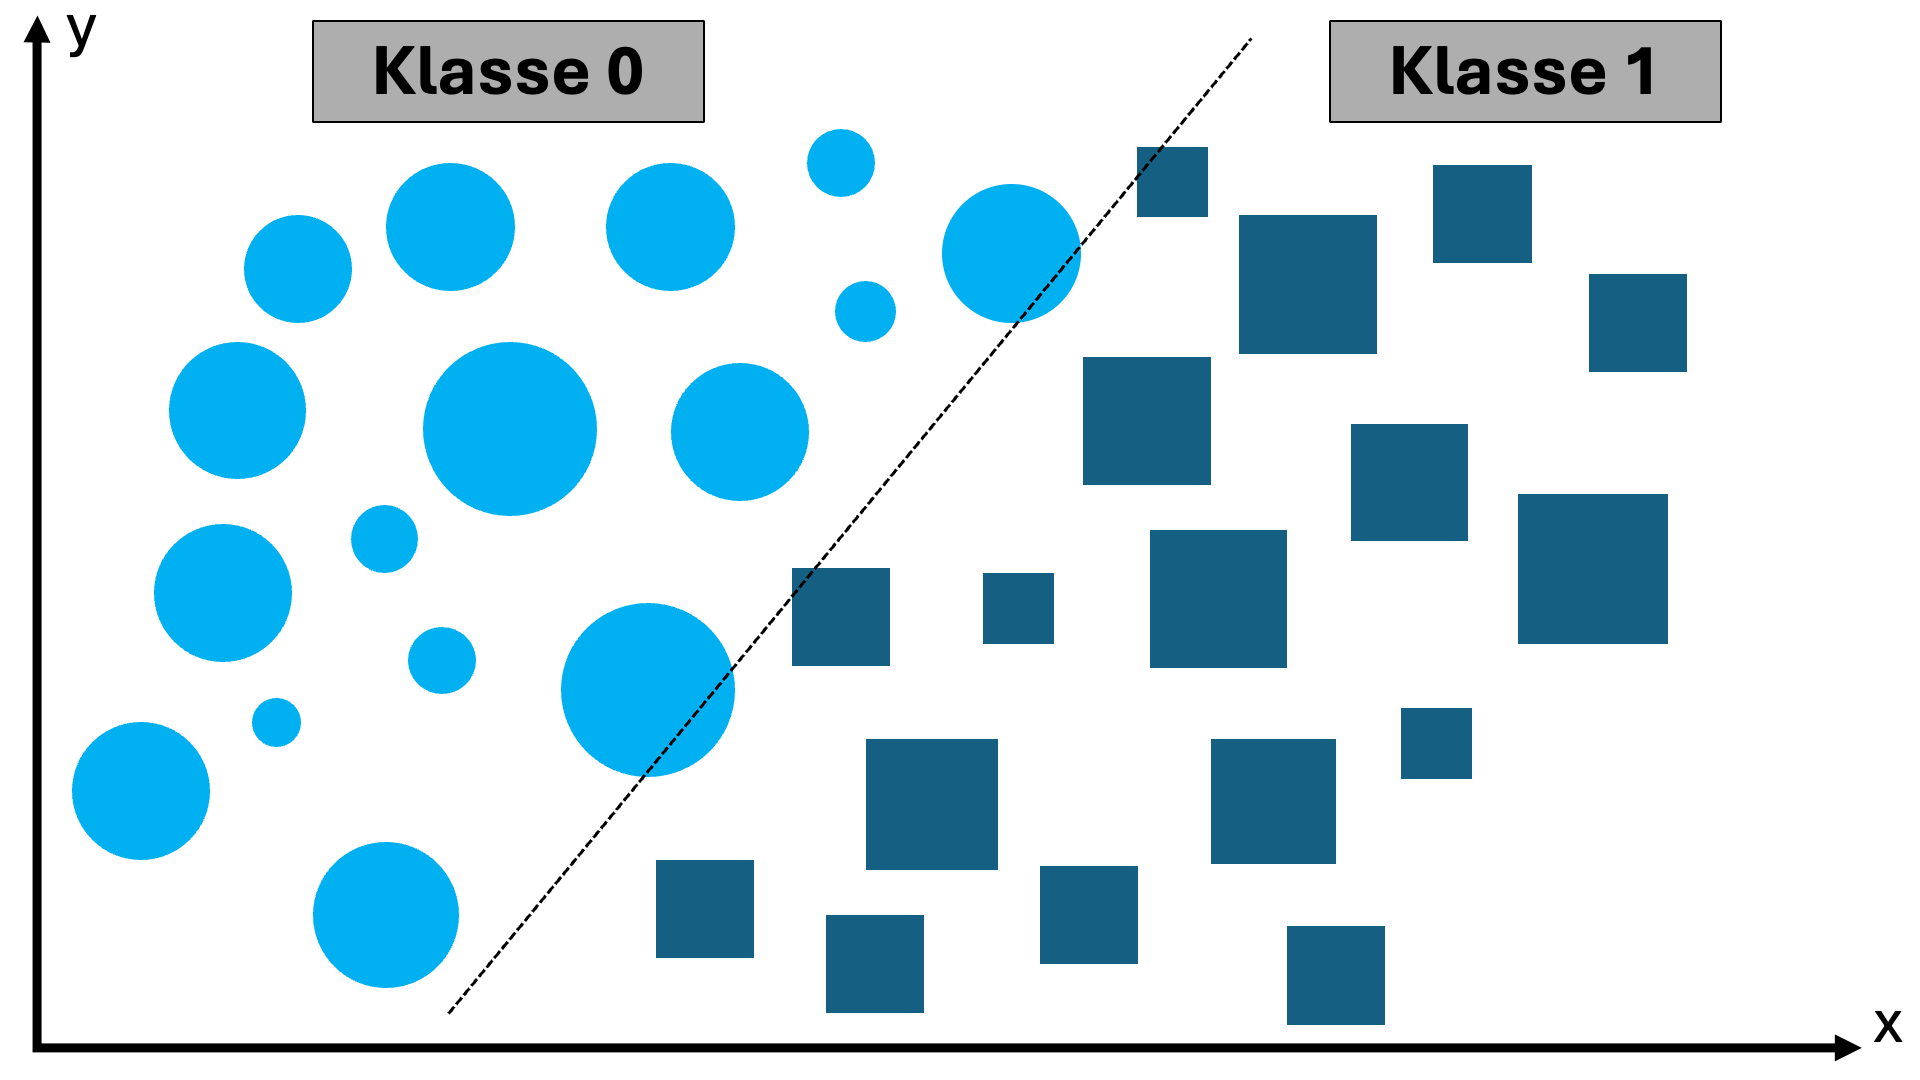
\includegraphics[width=\columnwidth]{binaere_klassifikation.png}}
    \caption{Schematische Darstellung der binären Klassifikation hier in form von Kreisen und Quadraten.}
    \label{fig:bin_class}
\end{figure}

Neben dem Training eigener Modelle können auch vortrainierte Modelle von Plattformen wie TensorFlow oder PyTorch geladen und fein abgestimmt werden.


\section{Datensatz} 
\label{sec:dataset}
In diesem Kapitel wird der verwendete Datensatz sowie die damit einhergehenden Herausforderungen beschrieben.

\subsection{Allgemeine Beschreibung des Datensatzes}
\label{sec:dataset_description}
Der Datensatz besteht aus ca. 2000 Bildern unterschiedlicher Qualität und Perspektive, die als JPEG-Dateien vorliegen. Zu jedem Bild existiert eine zugehörige Segmentierungsmaske im PNG-Format, die die Segmentierungsinformationen enthält. Zusätzlich enthält der Datensatz eine \texttt{tags.json}-Datei, die jedem Bild das Geschlecht der abgebildeten Person zuordnet. Die Geschlechterverteilung im Datensatz beträgt etwa 1200 Bilder von Männern und 800 Bilder von Frauen.

% Masken und Münder?
\subsection{Herausforderungen bei der Datenverarbeitung}  
Die Verarbeitung dieses Datensatzes bringt mehrere Herausforderungen mit sich. Die variierende Bildqualität und unterschiedlichen Perspektiven können die Konsistenz der Segmentierung beeinträchtigen und die Generalisierbarkeit von Modellen erschweren. Zudem liegt eine Ungleichverteilung der Geschlechter mit 1200 Bildern von Männern und 800 von Frauen vor, was zu Verzerrungen in geschlechtsspezifischen Analysen führen kann. 

Die Qualität und Konsistenz der Segmentierungsmasken ist ein weiterer kritischer Faktor, da ungenaue oder fehlerhafte Masken ungewollte Fehler bei der Vorverarbeitung hervorrufen können. Auch die Labels in der \texttt{tags.json}-Datei können Ungenauigkeiten enthalten, welche zu fehlern im Training des CNNs führen können. 
%Darüber hinaus erfordert die Verarbeitung von 2000 Bildern und Masken erhebliche Rechenleistung und Speicherplatz. 

Je nach Anwendung könnten weitere Herausforderungen auftreten, etwa wenn die Qualität der Segmentierung oder die Vielfalt der Perspektiven die Leistung eines Erkennungsmodells beeinträchtigt. % Warum ist dieser Absatz drin? 

\section{Implementierte Lösung}

\begin{figure}[H]
    \centerline{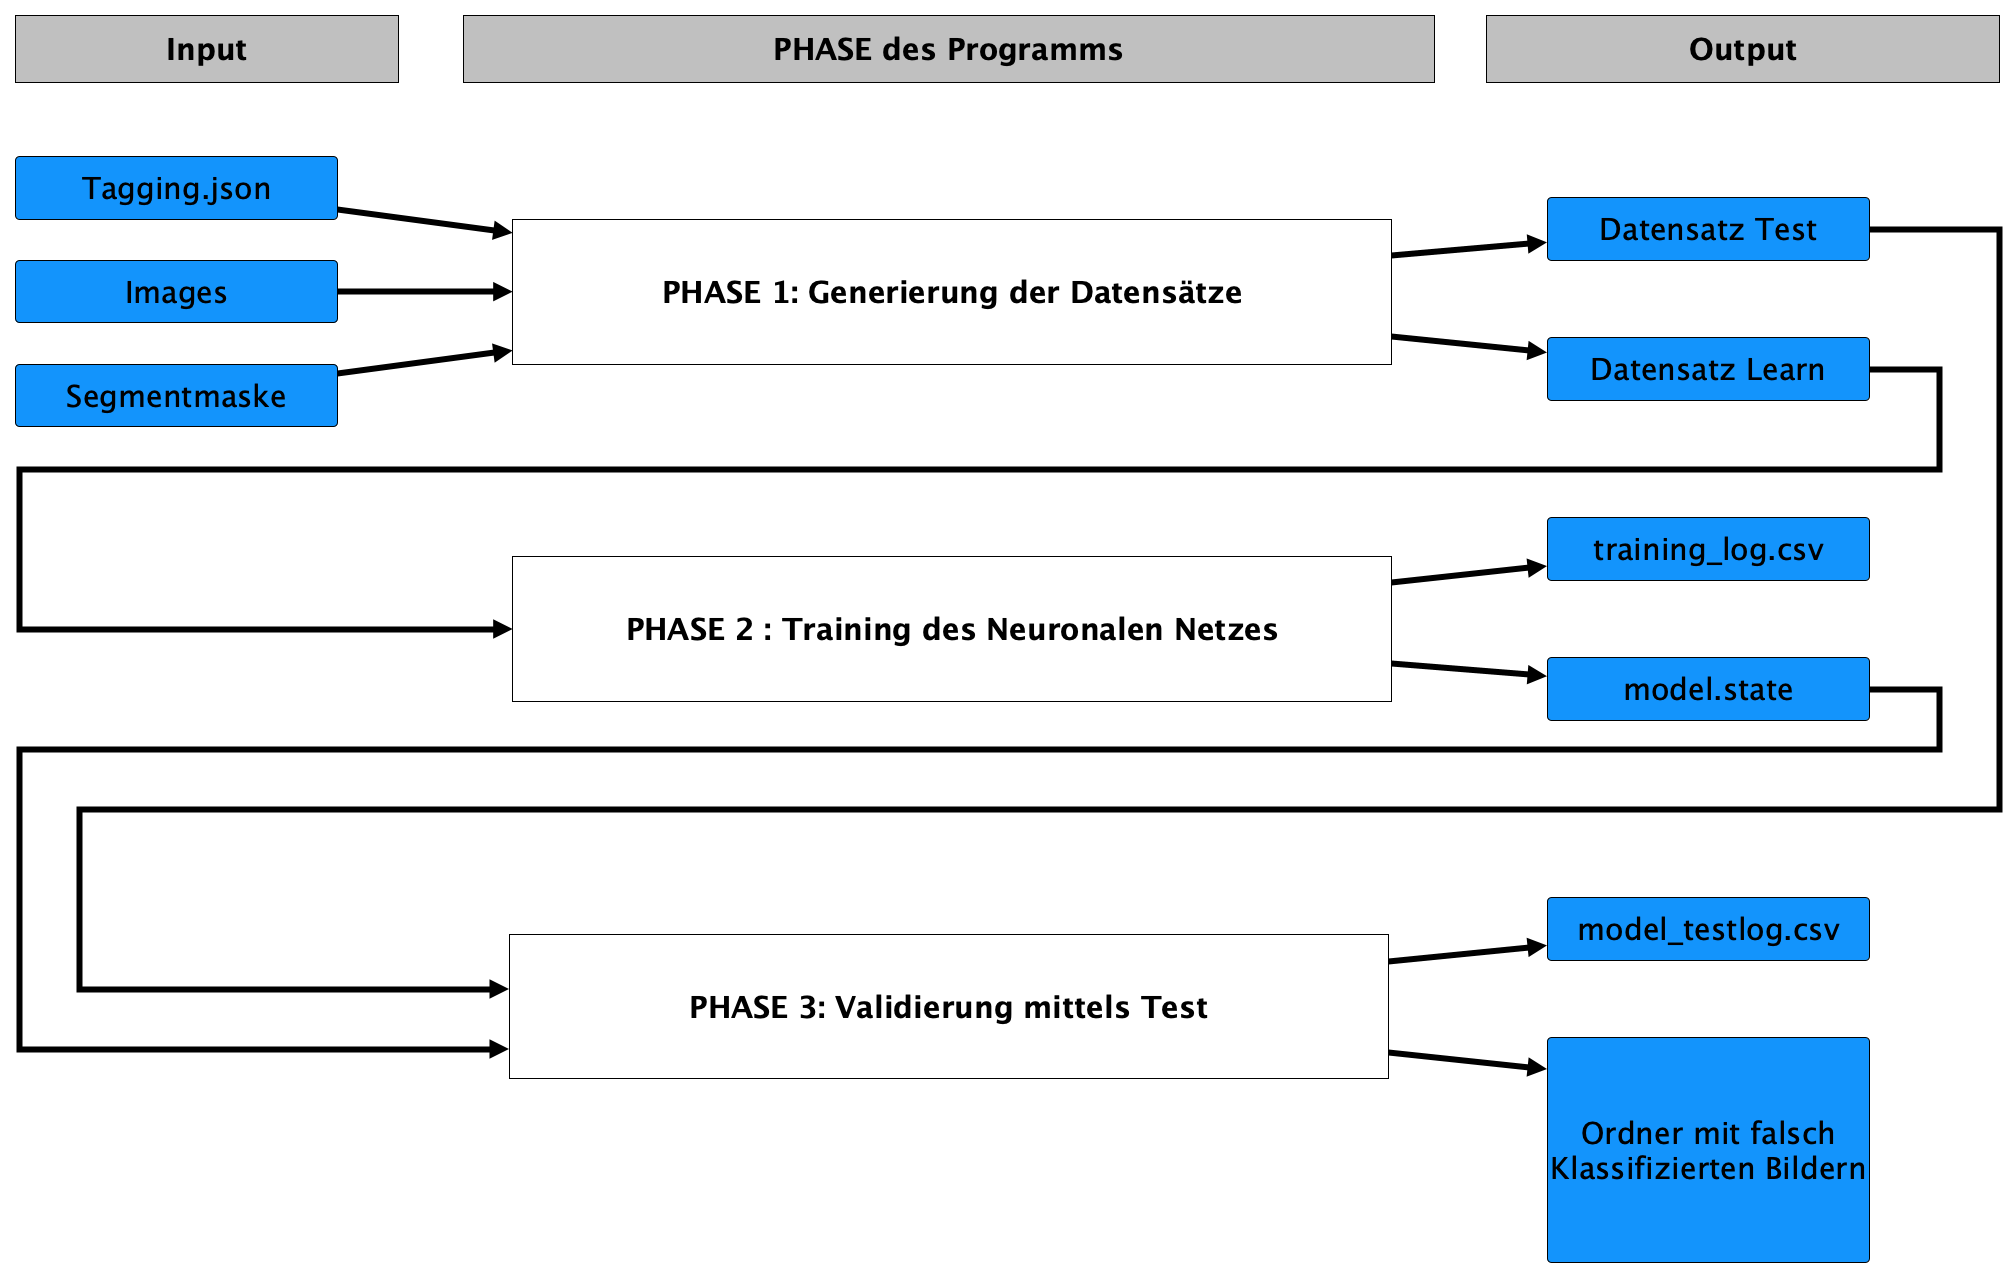
\includegraphics[width=\columnwidth]{Architektur.png}}
    \caption{Darstellung der Programmarchitektur in Form eines Blockschaltbildes.}
    \label{fig:architecture}
\end{figure}

Der in Abbildung \ref{fig:architecture} vereinfacht dargestellte Workflow veranschaulicht die Implementierung des Lösungsvorschlags zu der Aufgabe Geschlechterklassifikation mit dem in Kapitel \ref{sec:dataset} beschriebenen Datensatz. Im Folgenden wird der Lösungsvorgang detailliert beschrieben.

\subsection{Generierung der Daten}
Die in der Datei \texttt{data\_generation.py} implementierten Funktionen lesen den in Kapitel \ref{sec:dataset_description} beschriebenen Datensatz ein und verarbeiten die Bilder mittels der Segmentierungsmasken. Dabei wird den Bildern eine zusätzliche Farbebene (Alpha-Kanal) hinzugefügt und die abgebildete Person freigestellt. Das resultierende Bild wird mittels einer affinen Transformation in eine einheitliche Position und Ausrichtung gebracht. Hierzu werden die Schwerpunkte der Konturen von Augen und Mund extrahiert und für die Berechnung der Transformationsmatrix bereitgestellt. Anschließend werden die Bilder in einem neuen Verzeichnis gespeichert, um sie für das Training und Test des Modells zu verwenden.

\subsection{Training des Modells}
\label{sec:training}
Das Training des neuronalen Netzwerks erfolgt mit den in der Datei \texttt{classification.py} implementierten Funktionen und Methoden. Dabei wird das Modell über mehrere Epochen hinweg mit dem generierten Datensatz trainiert. Die Trainingsdaten werden in Batches geladen und dem Modell übergeben. Nach jeder Epoche wird das Modell anhand eines Validierungsdatensatzes evaluiert, um die Genauigkeit der Klassifikation zu überprüfen. Während des iterativen Trainingsprozesses werden die Modellgewichte durch die Optimierungsfunktionen kontinuierlich angepasst, um die Klassifikationsgenauigkeit zu maximieren. Nach Abschluss des Trainings wird das trainierte Modell gespeichert und für die spätere Verwendung bereitgestellt. 

Zur Vermeidung von Overfitting - also der Überanpassung des Modells an irrelevante Merkmale der Trainingsdaten - werden die Methoden der Data Augmentation und des Early Stopping eingesetzt. Overfitting führt dazu, dass das Modell spezifische Eigenschaften der Trainingsdaten memoriert, anstatt generalisierbare Muster zu erkennen, wodurch seine Leistungsfähigkeit auf unbekannten Daten und damit seine Generalisierbarkeit eingeschränkt wird.

Data Augmentation beschreibt die gezielte Veränderung der Trainingsdaten, um deren Vielfalt zu erhöhen. Dadurch wirkt der Datensatz größer, als er tatsächlich ist. 

Early Stopping beschreibt das automatische Abbrechen des Trainings, wenn sich die Genauigkeit des Modells auf den Validierungsdaten nicht weiter verbessert.


\begin{figure}[H]
    \centerline{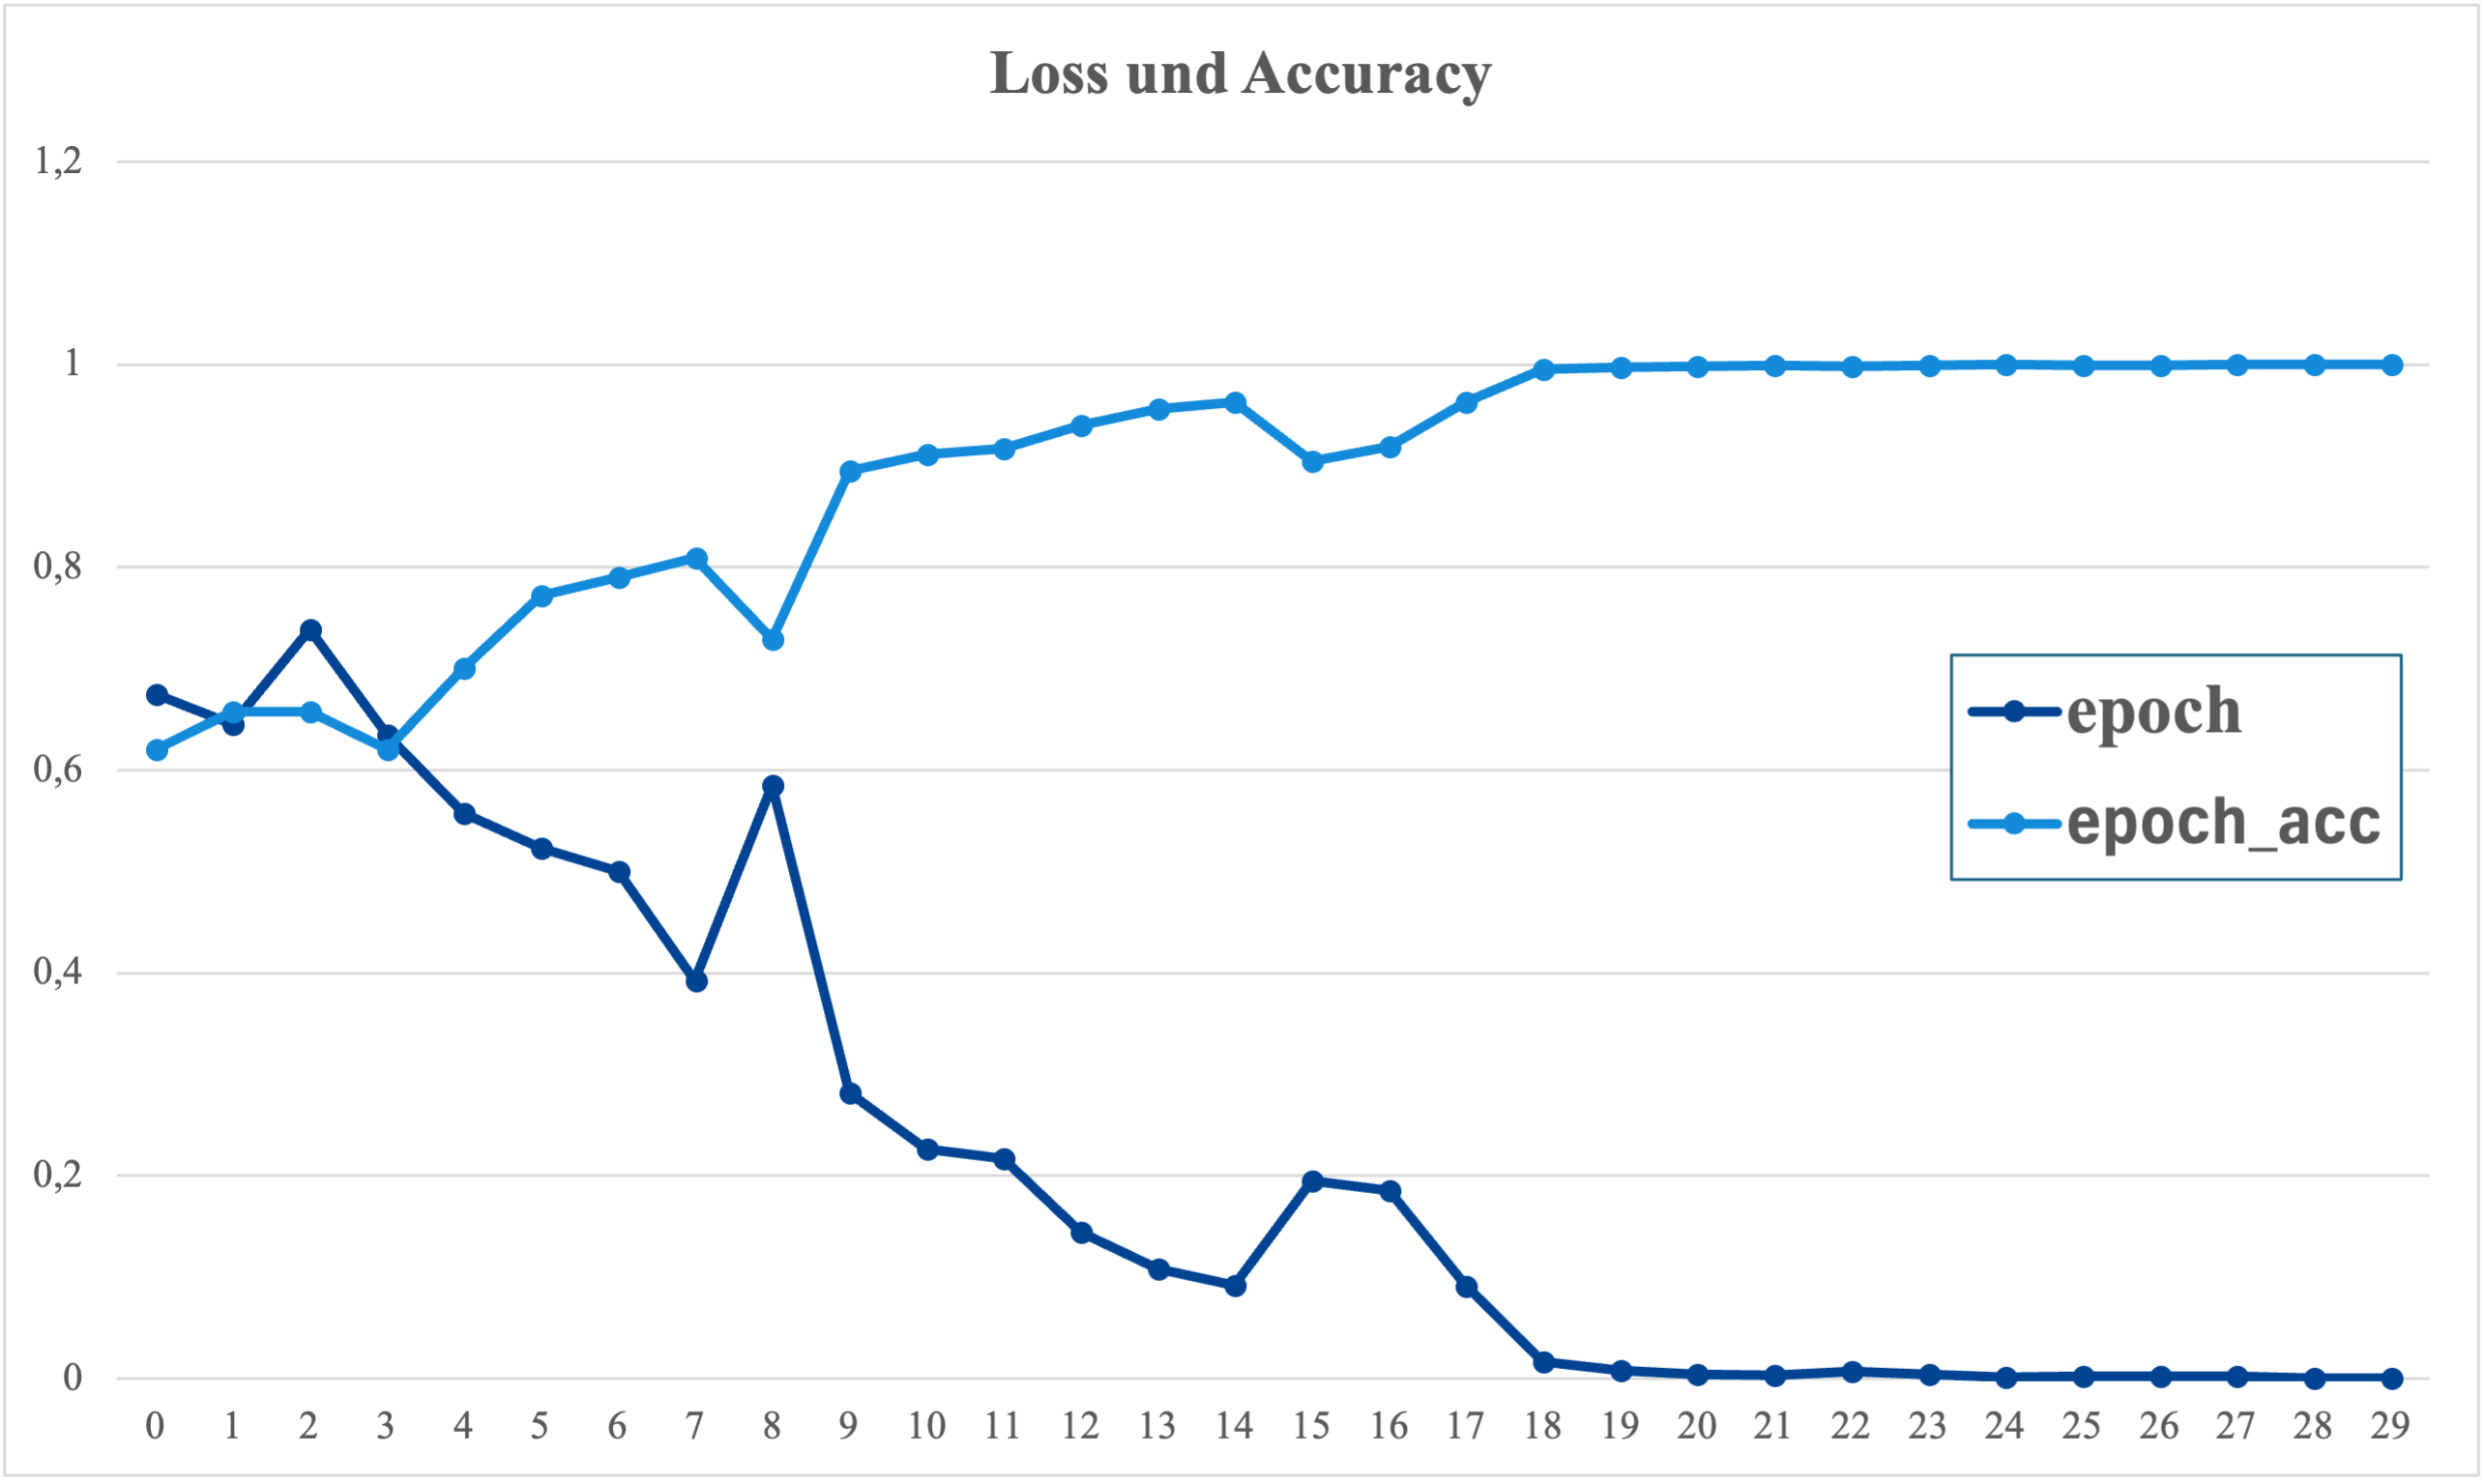
\includegraphics[width=\columnwidth]{Trainingslog.png}}
    \caption{Trainingsergebnis pro Epoche des finalen Modells.}
    \label{fig:trainlog}
\end{figure}

Die Abbildung \ref{fig:trainlog} zeigt das Trainingsergebnis des finalen Modells. Die Klassifikationsgenauigkeit des Modells steigt mit jeder Epoche und nähert sich einem Wert von $100 \%$ asymptotisch an. Zudem verringert sich der Verlust, bis dieser nahezu $0 \%$ erreicht. Dies zeigt, dass das Modell gut trainiert ist und eine hohe Genauigkeit in der Geschlechterklassifikation erzielt.

%Zudem lässt sich in der Grafik erkennen, zu welchen Zeitpunkten die Data Augmentation angewendet wird. In diesen Phasen treten kurzzeitige Verschlechterungen der Genauigkeit und ein Anstieg des Verlusts auf, was auf die gezielte Modifikation des Datensatzes zurückzuführen ist.

%Den Absatz hab ich gekillt, weil das nicht so ganz richtig ist und sooooo wichtig ist es nicht. 

\subsection{Test des Modells}
Das in Kapitel \ref{sec:training} trainierte und gespeicherte Modell wird für die Testphase neu geladen. Durch dieses erneute Laden des Modells wird sichergestellt, dass das Modell unabhängig von dem Trainingsprozess evaluiert wird.

Hierbei wird dem Modell der Testdatensatz übergeben. Dieser enthält für das Modell unbekannte Daten und ermöglicht somit eine objektive Bewertung der Modellleistung. Die Klassifikationsergebnisse werden mit den tatsächlichen Labels verglichen, um die Genauigkeit des Modells zu bestimmen. Das Ergebnis wird in Form einer Erfolgsquote ausgegeben, die in Prozent die Anzahl der korrekt klassifizierten Bilder im Verhältnis zur Gesamtanzahl der Testbilder angibt.

Zudem werden die falsch klassifizierten Bilder in ein separates Verzeichnis gespeichert, um eine gezielte Fehleranalyse zu ermöglichen. %Brauchen wir den Absatz?


\subsection{Ausführung des Python Codes}

In diesem Abschnitt wird beschrieben, wie der mit diesem Paper abgegebene Python-Code ausgeführt werden kann.

Um die vollständige Pipeline der Datenverarbeitung, das Training des Modells und den anschließende Test durchzuführen, muss die Datei \texttt{classification.py} ausgeführt werden. Dazu müssen alle drei Skripte im selben Verzeichnis liegen.

Im selben Verzeichnis wie die Datei \texttt{classification.py} muss sich ebenfalls ein Verzeichnis \texttt{Images} befinden, in welchem der unsortierte Datensatz mit Segmentierungsmasken abgelegt sein muss.

Während der Verarbeitung wird automatisch ein Ordner \texttt{Datensatz} erstellt, der die sortierten Bilder enthält und in zwei Unterordner \texttt{Train} und \texttt{Test} unterteilt wird.

Sollte es beim Ausführen des Codes zu Problemen kommen, kann dies darauf hindeuten, dass die benötigten Bibliotheken nicht installiert sind. Diese können mit dem Befehl \texttt{pip install -r requirements.txt} installiert werden.

Falls ausschließlich das trainierte Modell getestet werden soll, können die Funktionen \texttt{train\_model()} und \texttt{dg.preprocess()} in der Datei \texttt{classification.py} auskommentiert werden.


\section{Lösungsansätze im Vergleich}
In diesem Kapitel werden fünf Ansätze zur Implementierung des \ac{cnn} vorgestellt. Insgesamt umfasst die Versuchsreihe 23 trainierte neuronale Netze unterschiedlicher Einstellungen und Dimensionen.

% Um die zentralen Erkenntnisse und den Fortschritt über die Trainingsphasen hinweg darzustellen, wurden fünf repräsentative Modelle ausgewählt. Diese Modelle verdeutlichen sowohl die Entwicklung der Klassifikationsgenauigkeit als auch den Einfluss der gewählten Architektur auf die Trainingsdauer und die Generalisierungsfähigkeit des Netzwerks.

\subsection{Ablauf der Optimierung}
\label{sec:optimization}
Die Grundlage für das Design des neuronalen Netzes bildet ein im Labor verwendeter PyTorch-Code. Dieser Code ist in seinen Parametern ergänzt, um den verwendeten Bildgrößen und Bildkanälen gerecht zu werden. 

\begin{figure}[H]
    \centerline{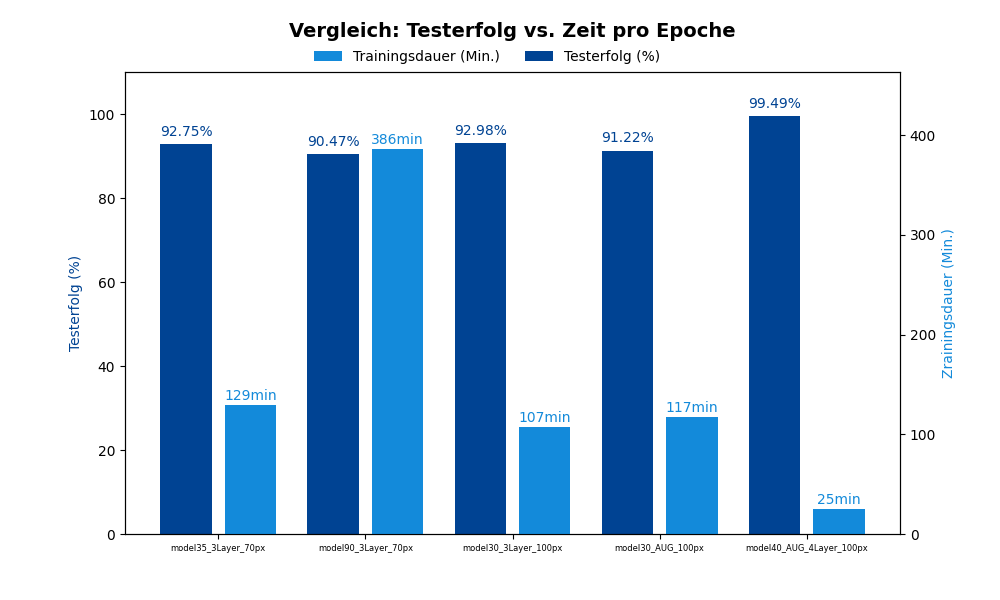
\includegraphics[width=\columnwidth]{Erfolg_Dauer.png}}
    \caption{Vergleich der Testgenauigkeit der jeweiligen Modelle in Abhängigkeit von der Dauer einer Trainingsepoche.}
    \label{fig:compareGraph}
\end{figure}

Mit diesem ersten Programmentwurf entsteht unter anderem das Netz (Model35\_3Layer\_70px), welches zunächst den besten Wert im Test liefert. Dieses Modell ist mit drei Faltungsebenen und einer Reduktion auf 232960 linearen Datenpunkten ausgestattet.
Es wurde für den Test in 35 Epochen trainiert und liefert $92,7\%$ Genauigkeit im Test (siehe Abbildung \ref{fig:compareGraph}).

Der erste Optimierungsansatz besteht in der Erhöhung der Trainingsepochen. Bei gleichbleibenden Modellparametern wird das Netz mit 90 statt 35 Epochen trainiert. Dies hat maßgeblichen Einfluss auf die Gesamtdauer, die mit 386 Minuten deutlich über den 129 Minuten des Vorgängers liegt (siehe Abbildung \ref{fig:compareGraph}), ohne dabei eine Verbesserung der Testgenauigkeit zu bewirken.

\begin{figure}[H]
    \centerline{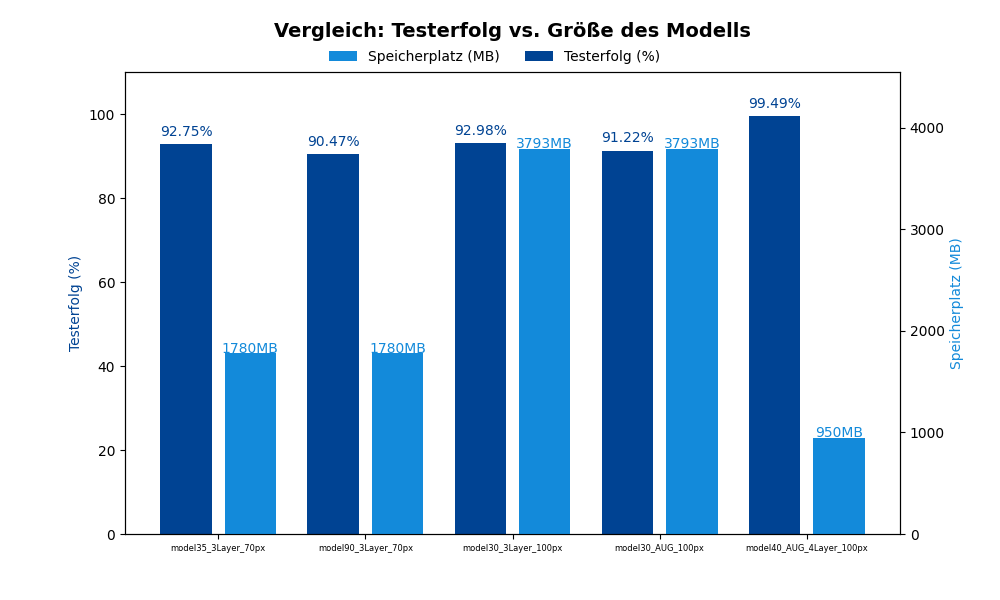
\includegraphics[width=\columnwidth]{Erfolg_Groesse.png}}
    \caption{Vergleich der Testgenauigkeit verschiedener Modelle in Abhängigkeit vom benötigten Speicherplatz.}
    \label{fig:compareSize}
\end{figure}

Der nächste Optimierungsansatz besteht in der Erhöhung der Bildauflösung. Der zuvor definierte Augenabstand von 70 Pixeln wird auf 100 Pixel erhöht, was eine Erhöhung der Bildauflösung von \(210\times280\)Pixeln auf \(300\times400\) Pixeln bedeutet. Der Augenabstand ist hierbei die maßgebliche Größe für die Segmentierung und Transformation der Bilder.

Diese Anpassung führt zu einer Steigerung der Modellkomplexität, da die zuvor verwendeten 232960 Datenpunkte nun auf 473600 erhöht wurden. 
Durch die zusätzlichen Informationen ist eine Steigerung des Erfolges um $0,2\%$ möglich. Mit der Erhöhung der Modellkomplexität und damit auch der Kapazität auf nahezu das Doppelte (siehe Abbildung \ref{fig:compareSize}), wird jedoch die Problematik des Overfittings besonders relevant und erfordert eine genauere Analyse.

Um dieser Problematik entgegenzuwirken, wurden die im Kapitel \ref{sec:training} vorgestellten Konzepte Data Augmentation und Early Stopping in den Programmcode implementiert.

Das daraus resultierende Modell (model30\_AUG\_3Layer\_100px) erzielt trotz Augmentation keine Verbesserung des Trainingserfolges, sondern verschlechtert diesen mit $91,22 \%$. 

Ohne den Augmentation-Ansatz zu verwerfen, besteht die nächste Optimierung in der Ergänzung einer weiteren Faltungsebene. Dies reduziert die linearen Parameter und damit auch die Komplexität des Modells, was sich positiv auf die Trainingsdauer auswirkt. In einem ersten Test erziehlt dieses letzte Modell (model40\_AUG\_3Layer\_100px\_ES) zunächst $94 \%$ und in einem zweiten Test $99 \%$.

\subsection{Diskussion der Lösungsansätze}
Alle drei Lösungsansätze bieten solide Ergebnisse für das Klassifikationsproblem. Keines der vorgestellten Modelle liefert Ergebnisse schlechter als $90\%$. Hinsichtlich der Komplexität und der benötigten Rechenressourcen zeigt sich jedoch, dass das Modell mit Data Augmentation und einer zusätzlichen Faltungsebene (model40\_AUG\_3Layer\_100px\_ES) die besten Resultate erzielt. Es kombiniert eine hohe Genauigkeit mit der kürzesten Trainingsdauer und kleinsten Speicherplatzanforderung, was es zu einer effizienten und effektiven Lösung für die Geschlechterklassifikation macht (siehe Abbildung \ref{fig:compareGraph} und Abbildung \ref{fig:compareSize}).

Die anderen Modelle liefern hinsichtlich des Erfolges ebenfalls solide Resultate. 
Unter Berücksichtigung der zeitlichen Komponente des Optimierungsfortschrittes hinsichtlich des Codeaufbaus der fünf Modelle sind die anfangs erreichten $92,75 \%$ ebenfalls nicht zu vernachlässigen. Hier wurden $7\%$ beziehungsweise $1\%$ weniger erzielt als beim besten Modell, allerdings mit fünf Tagen weniger Arbeitsaufwand für die Codeoptimierung. Ob die $99\%$ tatsächlich aussagekräftig sind, bleibt fraglich, da die Datenbasis nicht ausreichend groß ist, um eine Generalisierung des Modells zu gewährleisten und das Ergebnis mit neu gemischten Datensätzen erreicht wurde.

Die dazwischen getesteten Modelle stellen verschiedene Optimierungsversuche dar, die im Laufe der Entwicklung durchgeführt wurden. Die Beschreibung dieser Optimierungen und deren Auswirkungen auf die Modellleistung sind im letzten Kapitel (Kapitel \ref{sec:optimization}) dokumentiert.

\section{Fazit}
\label{sec:conclusion}
In dieser Arbeit wurde die Verarbeitung und Klassifikation von Gesichtsaufnahmen zur Geschlechterklassifikation mittels neuronaler Netze untersucht. Der Wissensgewinn über die Zeit war erheblich, da verschiedene Modelle und Optimierungsansätze getestet und evaluiert wurden. Beginnend mit einem einfachen Modell, das bereits eine solide Genauigkeit erzielte, wurden durch schrittweise Optimierungen wie die Erhöhung der Bildauflösung, die Implementierung von Data Augmentation und Early Stopping sowie die Anpassung der Netzwerkarchitektur signifikante Verbesserungen erreicht.

%Die besten Ergebnisse wurden mit einem Modell erzielt, das Data Augmentation und eine zusätzliche Faltungsebene nutzte, was die Genauigkeit auf bis zu $99 \%$ steigerte. Dies zeigt, dass durch gezielte Optimierungen und Anpassungen erhebliche Leistungssteigerungen möglich sind. - Mag den Absatz nicht so, steht ja oben (Andi)

Als Ausblick soll nicht unerwähnt bleiben, dass weitere Verbesserungen durch den Einsatz fortschrittlicherer Aktivierungsfunktionen wie Sigmoid möglich gewesen wären. Diese könnten die Klassifikationsgenauigkeit weiter erhöhen, indem sie nichtlineare Beziehungen in den Daten besser modellieren. Zukünftige Arbeiten könnten sich darauf konzentrieren, diese und andere fortschrittliche Techniken zu integrieren, um die Modellleistung weiter zu optimieren.

Insgesamt zeigt diese Arbeit, dass durch iterative Optimierung und den Einsatz moderner Techniken in der Bildverarbeitung und im maschinellen Lernen robuste und leistungsfähige Modelle zur Geschlechterklassifikation entwickelt werden können.


\end{document}
